\chapter{Algoritmo Genético}
\section{Calibração com a base de dados TEC-II\_5-8}
Calibração do Algoritmo Genético - G.A. para Populações [\textit{Pop}] de 10 à 100 (intervalos de 10) e Gerações [\textit{Gen.}] de 100 à 1000 (intervalos de 100) avaliando o \textit{Fitness} [\textit{Fit.}] (Equação \ref{eq-fitness}) e o número de características selecionadas [N].

\begin{center}
\renewcommand\arraystretch{0.8}
\begin{longtable}{|cc|cc|cc|cc|cc|}
\hline
 &  & \multicolumn{2}{c}{Nota 100} &  \multicolumn{2}{c}{Nota 93} & \multicolumn{2}{c}{Nota 90} & \multicolumn{2}{c}{Nota 0} \vline \\
\textit{Pop.} & \textit{Gen.} & \textit{Fit.} & N &  \textit{Fit.} & N & \textit{Fit.} & N & \textit{Fit.} & N \\ \hline
\endhead
\hline
\multicolumn{3}{r}{{Continua na próxima página}} \\ 
\endfoot

\hline \hline
\multicolumn{3}{r}{{\'Ultima p\'agina}} \\
\endlastfoot
\input{tables/relatorio-ga.csv}

\hline
\end{longtable}
\captionof{table}{Calibração do Algoritmo Genético conforme os resultados da seleção de características para quatro classes [100, 93, 90 e 0].}
\label{tab-ga-calibracao}
\end{center}

\chapter{Processamento de Linguagem Natural}
\section{Lista de {\it Stopwords}}\label{stopwords}
Um dos processos para eliminação das informações que são irrelevantes quanto ao contexto e manutenção do conteúdo essencial do texto para interpretação foi a remoção de \textit{stopwords}. Essas, são palavras que podem estar presentes em qualquer texto e são utilizadas como conectivos textuais, sem grande ganho na interpretação dos fatos apresentados. A Tabela \ref{tab-stopwords-en} apresenta a lista de \textit{stopwords} para a língua inglesa enquanto a Tabela \ref{tab-stopwords-pt} contém a lista de \textit{stopwords} para a língua portuguesa.

\begin{table}[h]
\centering
\renewcommand\arraystretch{0.8}
\begin{tabular}{ccccc}
\hline
\multicolumn{5}{c}{Lista \textit{stopwords} para o Inglês} \\
\hline

\input{tables/stopwords-en.csv}

\hline
\hline
\end{tabular}
\caption{Lista de \textit{stopwords} utilizado no pré-processamento da língua inglesa.}
\label{tab-stopwords-en}
\end{table}

\begin{table}[h]
\centering
\renewcommand\arraystretch{0.8}
\begin{tabular}{ccccc}
\hline
\multicolumn{5}{c}{Lista de \textit{stopwords} para o Português} \\
\hline

\input{tables/stopwords-pt.csv}

\hline
\hline
\end{tabular}
\caption{Lista de \textit{stopwords} utilizado no pré-processamento da língua portuguesa.}
\label{tab-stopwords-pt}
\end{table}

\chapter{Experimentos}
\section{Base de Dados VestUfes}\label{sec-enunciados-vestufes}
Para a base de dados do Vestibular da Universidade Federal do Espírito Santo, são apresentados os enunciados das cinco atividades de português avaliadas em 2012. Essas atividades foram utilizadas por \cite{pissinati2014-master} para comparar sete modelos de avaliação semi-automática desenvolvidos com as correções de dois humanos especialistas. Cada atividade foi transcrita do documento original escrito à mão pelo aluno no vestibular. Ao total foram coletadas 92 atividades de cada questão, totalizando 460 respostas.

\subsection{Questão 1}
\textit{Ao elaborar um panorama da ficção contemporânea, Flávio Carneiro (No país do presente. Rio de Janeiro: Rocco, 2005. p. 305-311) elenca uma série de
traços de nossa literatura contemporânea, a saber: 1) o cruzamento da literatura com a linguagem da mídia e da internet; 2) a problematização das relações amorosas, em especial as femininas e homoeróticas; 3) a volta ao campo ou a cidades do interior; 4) o ressurgimento do narrador clássico, cujo relato beira
a oralidade; 5) a força da narrativa fantástica; 6) a multiplicação de textos de autoria e temática femininas; 7) a reescritura contínua das estórias; 8) o clima detetivesco; 9) a presença de fatos históricos; 10) o aumento de narrativas memorialísticas; 11) a ficção de cunho social; 12) a hegemonia de personagens
anônimos, comuns, anti-heroicos; 13) a mistura de gêneros, literários ou não; 14) o humor como recurso e técnica; 15) a influência do mercado editorial. Considerando um dos três romances seguintes: Boca do inferno, de Ana Miranda (1989); Ensaio sobre a cegueira, de José Saramago (1995); Kitty aos 22: divertimento, de Reinaldo Santos Neves (2006), indique, na obra escolhida, a ocorrência de pelo menos dois dos quinze traços acima citados e explique de
que modo eles ocorrem na narrativa.
}

\subsection{Questão 2}
Escolha uma das três obras seguintes: Romanceiro da Inconfidência, de Cecília Meireles; Vidas secas, de Graciliano Ramos; O noviço, de Martins Pena, e faça o que se pede: 

\begin{itemize}
\item Justifique o título da obra que você escolheu.
\item Explique a relevância do trecho da obra escolhida, abaixo transcrito, para a compreensão dessa obra.
\end{itemize}

TEXTO 1
 
Romance II ou Do ouro incansável

[...]

De seu calmo esconderijo,

o ouro vem, dócil e ingênuo;

torna-se pó, folha, barra,

prestígio, poder, engenho...

É tão claro! ? e turva tudo:

honra, amor e pensamento.

[...]

Mil galerias desabam;

mil homens ficam sepultos;

mil intrigas, mil enredos

prendem culpados e justos;

já ninguém dorme tranquilo,

que a noite é um mundo de sustos.

(Romanceiro da Inconfidência, de Cecília Meireles)

TEXTO 2

Que iriam fazer? Retardaram-se, temerosos. Chegariam a uma terra desconhecida e civilizada, ficariam presos nela. E o sertão continuaria a mandar gente
para lá. O sertão mandaria para a cidade homens fortes, brutos como Fabiano, sinha Vitória e os dois meninos. 
(Vidas secas, de Graciliano Ramos)

TEXTO 3

AMBRÓSIO : Senhores, denuncio-vos um criminoso.

MEIRINHO : É verdade que tenho aqui uma ordem contra um noviço...

MESTRE : ... Que já de nada vale. (Prevenção.)

TODOS : O Padre-Mestre!

MESTRE (para Carlos) : Carlos, o Dom Abade julgou mais prudente que lá não voltásseis. Aqui tens a permissão por ele assinada para saíres do convento.

CARLOS (abraçando-o) : Meu bom Padre-Mestre, este ato reconcilia-me com os frades.

MESTRE : E vós, senhoras, esperai da justiça dos homens o castigo deste malvado. (Para Carlos e Em ??lia:) E vós, meus filhos, sede felizes, que eu pedirei para todos (ao público:) indulgência!
 ?
AMBRÓSIO : Oh, mulheres, mulheres! (Execução.)

(O noviço, de Martins Pena).

\subsection{Questão 3}
Reescreva, com as devidas adaptaçõs, as duas últimas falas do personagem MESTRE, de O noviço (TEXTO 3 da 2ª QUESTÃO), fazendo uso do pronome VOCÊ ou VOCÊS, conforme o caso.

\subsection{Questão 4}
Leia os textos abaixo e faça o que se pede:

TEXTO 1

"O navio negreiro''

Negras mulheres, suspendendo às tetas

Magras crianças, cujas bocas pretas

Rega o sangue das mães:

Outras, moças... mas nuas, espantadas,

No turbilhão de espectros arrastadas,

Em ânsia e mágoa vãs.

(Castro Alves)

TEXTO 2

"7''

Eu não sou eu nem sou o outro,

Sou qualquer coisa de intermédio:

Pilar da ponte de tédio

Que vai de mim para o Outro.

(Mário de Sá-Carneiro)

TEXTO 3

"Os arredores florem''

Os arredores florem:

figos, nervos, libélulas

a criarem nas águas

os brevíssimos movimentos.

(Paulo Roberto Sodré)

\begin{itemize}
\item Escolha um dos textos acima ("O navio negreiro''; "7''; "Os arredores florem''), indique e explique a ocorrência de um dos seguintes aspectos: som (aliteração, assonância, paronomásia, etc.), sentido (metáfora, alegoria, ironia, etc.), ritmo (rima, métrica, tonicidade, etc.) ou representação (imagem, descrição, comparação, etc.).
\item Nos três versos iniciais do trecho de "O navio negreiro''(TEXTO 1), o sujeito do enunciado é "o sangue das mães''. Reescreva, em prosa, esses versos, iniciando o período com "O sangue das mães'', fazendo as adaptações que o texto requer e mantendo o sentido do texto original.
\end{itemize}

\subsection{Questão 5}
Com base nos elementos constitutivos do ato de comunicação, Roman Jakobson estabeleceu seis funções da linguagem (e a ênfase de cada uma delas): referencial (ênfase no assunto; no conteúdo), emotiva (ênfase no emissor; no sujeito), conativa (ênfase no receptor; no interlocutor), poética (ênfase na forma; na construção), metalinguística (ênfase no código; na autorreferência) e fática (ênfase no canal; no contato). 

Escolha um dos textos da Questão 4, indique e explique a ocorrência de uma dessas funções.

\newpage
\section{Base de Dados Disciplinas UFES} \label{sec-disciplinas-ufes}
Base de dados extraída de disciplinas da Universidade Federal do Espírito Santo entre 2015 e 2016. Dentre as atividades coletadas estão as disciplinas de Filosofia, Métodos e Técnicas de Pesquisa Científica - MTPC e Tecnologia da Informação II. A Tabela \ref{tab-exp-dis-ufes} mostra para cada atividade o identificador, o nome, a quantidade e o percentual referente da base de treinamento e total de submissões, total de características selecionadas pelo mapa de características, percentual referente à seleção e o total de características da base de dados.
\begin{center}
\renewcommand\arraystretch{0.6}
\begin{longtable}{r|ccccccc}
\hline
& & \multicolumn{3}{c}{Submissões} & \multicolumn{3}{c}{Características}
\\
\# & \textit{Dataset} & Treino & (em \%) & Total & Selecionadas & (em \%) & Total \\
\hline
\endhead
\hline
\multicolumn{3}{r}{{Continua na próxima página}} \\ 
\endfoot

\hline \hline
\multicolumn{3}{r}{{\'Ultima p\'agina}} \\
\endlastfoot
\input{tables/ufes-experimentos.csv}

\hline
\end{longtable}
\captionof{table}{\textit{Datasets} coletados em disciplinas da Universidade Federal do Espírito Santo com as respectivas informações de esforço de correção e redução de dimensionalidade.}
\label{tab-exp-dis-ufes}
\end{center}

A Tabela \ref{tab-exp-dis-ufes-classificacao} apresenta para todas as atividades dessa base de dados o desempenho de avaliação antes e depois do processo de seleção de características com as métricas de Erro Quadrático Médio - MSE e Erro Médio Absoluto - MAE, \textit{Accuracy} - ACC, \textit{Precision}, \textit{Recall} e F1 para os dois classificadores testados KNN e CBC.

\begin{landscape}
\renewcommand\arraystretch{0.5}
\begin{longtable}{r|cccccc|cccccc}
& \multicolumn{6}{|c|}{KNN} & \multicolumn{6}{|c}{CBC} \\
\textit{Dataset} & MSE & MAE & ACC  & \textit{Precision} & \textit{Recall} & F1 & MSE & MAE & ACC  & \textit{Precision} & \textit{Recall} & F1 \\ \hline
\endhead
\hline
\multicolumn{3}{r}{{Continua na próxima página}} \\ 
\endfoot

\hline \hline
\multicolumn{3}{r}{{\'Ultima p\'agina}} \\
\endlastfoot
\input{tables/ufes-classificacao.csv}

\hline
\end{longtable}
\captionof{table}{Avaliação da classificação para cada atividade da base de dados conforme 6 métricas e dois classificadores.}
\label{tab-exp-dis-ufes-classificacao}

\end{landscape}

A Tabela \ref{tab-exp-dis-ufes-features} apresenta para todas as atividades com mais de uma classe dessa base de dados o processo de seleção de características com número de documentos e características - inicial e final. Para cada classe dessas atividades com mais de um item é analisada a similaridade interna - SI inicial e final, o coeficiente de redução e o número de características de classe.

\begin{center}
\renewcommand\arraystretch{0.8}
\begin{longtable}{r|cccc}
\hline
Dataset & C. Final & & Documentos & C. Inicial \\ \hline
\endhead
\hline
\multicolumn{3}{r}{{Continua na próxima página}} \\ 
\endfoot

\hline \hline
\multicolumn{3}{r}{{\'Ultima p\'agina}} \\
\endlastfoot
\input{tables/ufes-reducao-por-classe.csv}

\hline
\end{longtable}
\captionof{table}{Similaridade interna anterior e posterior à seleção de características em atividades da base de dados com mais de uma classe de nota.}
\label{tab-exp-dis-ufes-features}
\end{center}

Dada a expectativa de aumento de similaridade interna para melhoria do processo de avaliação, visualizamos nas figuras à seguir o aumento de similaridade interna da classe para cada nota representada na Tabela \ref{tab-exp-dis-ufes-features}.
\begin{figure}
\centering
\begin{minipage}{.3\textwidth}
  \centering
  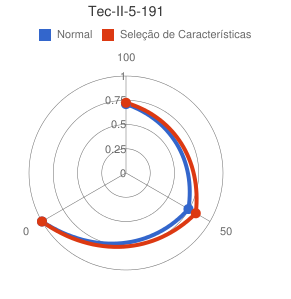
\includegraphics[width=\linewidth]{img/red-ufes-moodle/image1.png}
\end{minipage}%
\begin{minipage}{.3\textwidth}
  \centering
  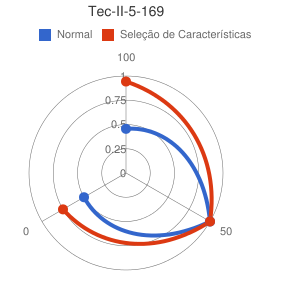
\includegraphics[width=\linewidth]{img/red-ufes-moodle/image2.png}
\end{minipage} %
\begin{minipage}{.3\textwidth}
  \centering
  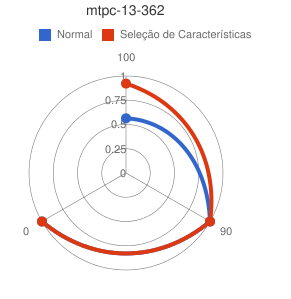
\includegraphics[width=\linewidth]{img/red-ufes-moodle/image3.png}
\end{minipage}
\begin{minipage}{.3\textwidth}
  \centering
  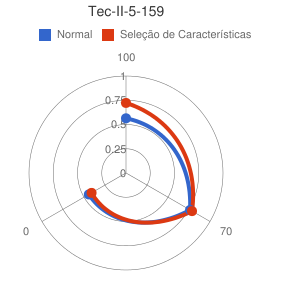
\includegraphics[width=\linewidth]{img/red-ufes-moodle/image4.png}
\end{minipage}%
\begin{minipage}{.3\textwidth}
  \centering
  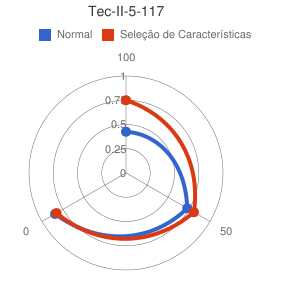
\includegraphics[width=\linewidth]{img/red-ufes-moodle/image5.png}
\end{minipage} %
\begin{minipage}{.3\textwidth}
  \centering
  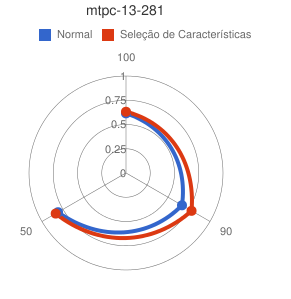
\includegraphics[width=\linewidth]{img/red-ufes-moodle/image6.png}
\end{minipage}
\begin{minipage}{.3\textwidth}
  \centering
  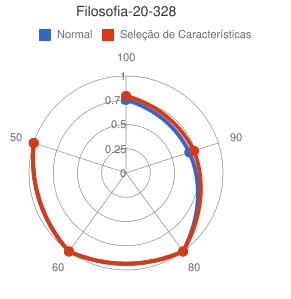
\includegraphics[width=\linewidth]{img/red-ufes-moodle/image7.png}
\end{minipage}%
\begin{minipage}{.3\textwidth}
  \centering
  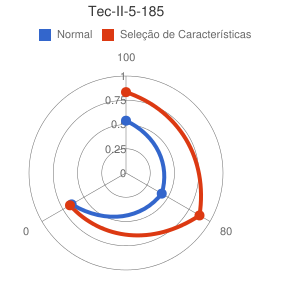
\includegraphics[width=\linewidth]{img/red-ufes-moodle/image8.png}
\end{minipage} %
\begin{minipage}{.3\textwidth}
  \centering
  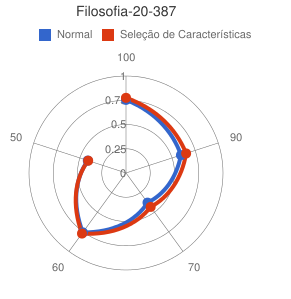
\includegraphics[width=\linewidth]{img/red-ufes-moodle/image9.png}
\end{minipage}
\begin{minipage}{.3\textwidth}
  \centering
  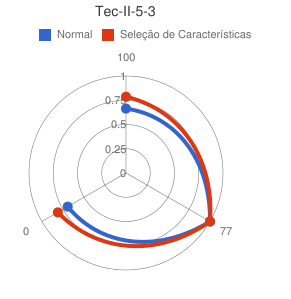
\includegraphics[width=\linewidth]{img/red-ufes-moodle/image10.png}
\end{minipage}%
\begin{minipage}{.3\textwidth}
  \centering
  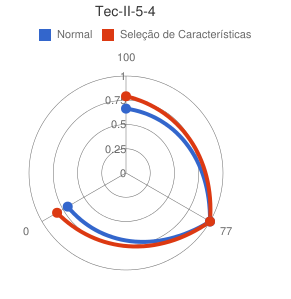
\includegraphics[width=\linewidth]{img/red-ufes-moodle/image11.png}
\end{minipage} %
\begin{minipage}{.3\textwidth}
  \centering
  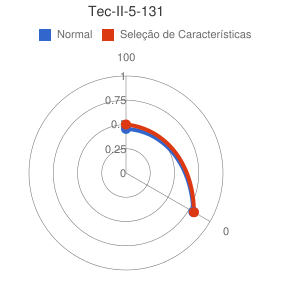
\includegraphics[width=\linewidth]{img/red-ufes-moodle/image12.png}
\end{minipage}
\caption{Gráficos para aumento de similaridade por nota.}
\end{figure}

\begin{figure}
\centering
\begin{minipage}{.3\textwidth}
  \centering
  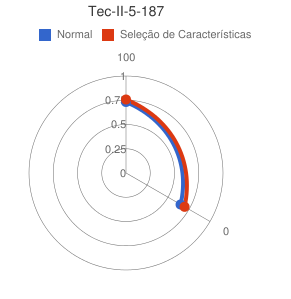
\includegraphics[width=\linewidth]{img/red-ufes-moodle/image13.png}
\end{minipage}%
\begin{minipage}{.3\textwidth}
  \centering
  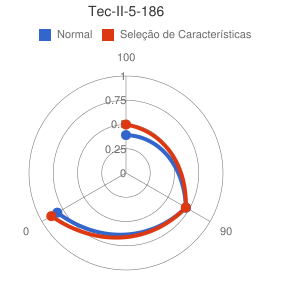
\includegraphics[width=\linewidth]{img/red-ufes-moodle/image14.png}
\end{minipage} %
\begin{minipage}{.3\textwidth}
  \centering
  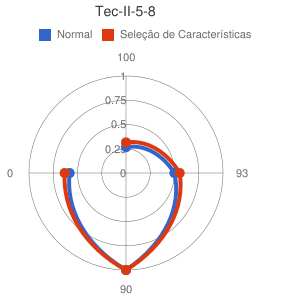
\includegraphics[width=\linewidth]{img/red-ufes-moodle/image15.png}
\end{minipage}
\begin{minipage}{.3\textwidth}
  \centering
  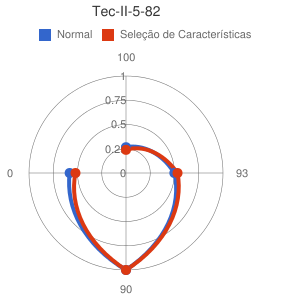
\includegraphics[width=\linewidth]{img/red-ufes-moodle/image16.png}
\end{minipage}%
\begin{minipage}{.3\textwidth}
  \centering
  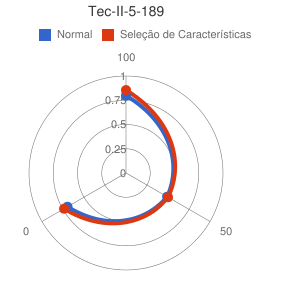
\includegraphics[width=\linewidth]{img/red-ufes-moodle/image17.png}
\end{minipage} %
\begin{minipage}{.3\textwidth}
  \centering
  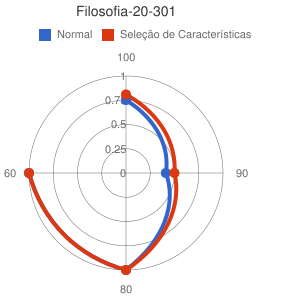
\includegraphics[width=\linewidth]{img/red-ufes-moodle/image18.png}
\end{minipage}
\begin{minipage}{.3\textwidth}
  \centering
  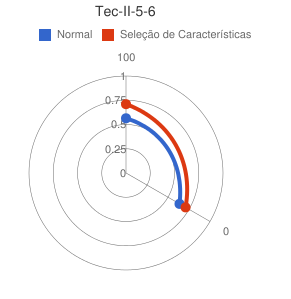
\includegraphics[width=\linewidth]{img/red-ufes-moodle/image19.png}
\end{minipage}%
\begin{minipage}{.3\textwidth}
  \centering
  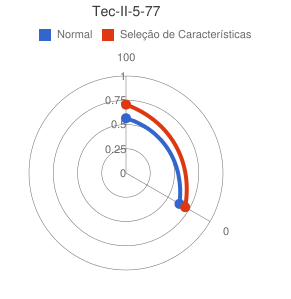
\includegraphics[width=\linewidth]{img/red-ufes-moodle/image20.png}
\end{minipage} %
\begin{minipage}{.3\textwidth}
  \centering
  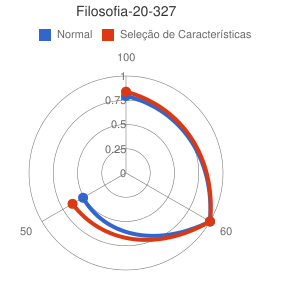
\includegraphics[width=\linewidth]{img/red-ufes-moodle/image21.png}
\end{minipage}
\caption{Gráficos para aumento de similaridade por nota das atividades da base de dados de Disciplinas da UFES.}
\end{figure}

\newpage
\section{Base de Dados Ciência da Computação UNT} \label{sec-DS-CC-UNT}
Base de dados extraída de atividades da disciplina de Estrutura de Dados para a Ciência da Computação da Universidade do Norte do Texas. Foram aplicadas dez listas de exercícios com sete questões cada e duas provas com dez questões. Os dados foram coletados por \cite{mohler2011} e contou com 30 alunos na disciplina. A Tabela \ref{tab-exp-dis-ufes} mostra para cada atividade o identificador, o nome, a quantidade e o percentual referente da base de treinamento e total de submissões, total de características selecionadas pelo mapa de características, percentual referente à seleção e o total de características da base de dados.

\begin{center}
\renewcommand\arraystretch{0.6}
\begin{longtable}{r|ccccccc}
\hline
& & \multicolumn{3}{c}{Submissões} & \multicolumn{3}{c}{Características}
\\
\# & \textit{Dataset} & Treino & (em \%) & Total & Selecionadas & (em \%) & Total \\
\hline
\endhead
\hline
\multicolumn{3}{r}{{Continua na próxima página}} \\ 
\endfoot

\hline \hline
\multicolumn{3}{r}{{\'Ultima p\'agina}} \\
\endlastfoot
\input{tables/mohler-experimentos.csv}

\hline
\end{longtable}
\captionof{table}{\textit{Datasets} coletados por \cite{mohler2011} em turmas de Ciência da Computação durante as aulas de Estrutura de Dados na Universidade do Norte do Texas.}
\label{tab-exp-mohler}
\end{center}

A Tabela \ref{tab-exp-mohler-classificacao} apresenta para todas as atividades dessa base de dados o desempenho de avaliação antes e depois do processo de seleção de características com as métricas de Erro Quadrático Médio - MSE e Erro Médio Absoluto - MAE, \textit{Accuracy} - ACC, \textit{Precision}, \textit{Recall} e F1 para os dois classificadores testados KNN e CBC.

\begin{landscape}
\renewcommand\arraystretch{0.5}
\begin{longtable}{r|cccccc|cccccc}
& \multicolumn{6}{|c|}{KNN} & \multicolumn{6}{|c}{CBC} \\
\textit{Dataset} & MSE & MAE & ACC  & \textit{Precision} & \textit{Recall} & F1 & MSE & MAE & ACC  & \textit{Precision} & \textit{Recall} & F1 \\ \hline
\endhead
\hline
\multicolumn{3}{r}{{Continua na próxima página}} \\ 
\endfoot

\hline \hline
\multicolumn{3}{r}{{\'Ultima p\'agina}} \\
\endlastfoot
\input{tables/mohler-classificacao.csv}

\hline
\end{longtable}
\captionof{table}{Avaliação da classificação para cada atividade da base de dados conforme 6 métricas e dois classificadores.}
\label{tab-exp-mohler-classificacao}
\end{landscape}

A Tabela \ref{tab-exp-mohler-features} apresenta para todas as atividades com mais de uma classe dessa base de dados o processo de seleção de características com número de documentos e características - inicial e final. Para cada classe dessas atividades com mais de um item é analisada a similaridade interna - SI inicial e final, o coeficiente de redução e o número de características de classe.

\begin{center}
\renewcommand\arraystretch{0.8}
\begin{longtable}{r|cccc}
\hline
\textit{Dataset} & C. Final & & Documentos & C. Inicial \\ \hline
\endhead
\hline
\multicolumn{3}{r}{{Continua na próxima página}} \\ 
\endfoot

\hline \hline
\multicolumn{3}{r}{{\'Ultima p\'agina}} \\
\endlastfoot
\input{tables/mohler-reducao-por-classe.csv}

\hline
\end{longtable}
\captionof{table}{Similaridade interna anterior e posterior à seleção de características em atividades da base de dados com mais de uma classe de nota.}
\label{tab-exp-mohler-features}
\end{center}

\newpage
\section{Caracterização das Questões Curtas}
O tamanho das respostas representa o conteúdo e adiciona dificuldades na avaliação sem conhecimento prévio da base da atividade. Assim, para todas as bases de dados é realizada a descrição das atividades quanto ao tamanho das respostas e da base de dados. Na Tabela \ref{tab-tamanho-respostas} é apresentada a dimensionalidade (número de características x número de documentos) e o tamanho das respostas segundo a média ($\overline{x}$), desvio padrão ($\sigma$) e a maior (máx) e menor (min) norma dos vetores de resposta.
\begin{center}
\renewcommand\arraystretch{0.8}
\begin{longtable}{l|cc|cccc|}
& & & \multicolumn{4}{|c|}{Submissões (em palavras)} \\
\textit{Dataset} & N. Documentos & N. Características & $ \overline{x} $ & $ \sigma $ & máx.  & min.  \\ \hline
\endhead
\hline
\multicolumn{3}{r}{{Continua na próxima página}} \\ 
\endfoot

\hline \hline
\multicolumn{3}{r}{{\'Ultima p\'agina}} \\
\endlastfoot

\input{tables/tam-vest.csv}

\input{tables/tam-disciplinas.csv}

\input{tables/tam-unt.csv}

\input{tables/tam-kaggle.csv}

\hline
\end{longtable}
\captionof{table}{Tamanho dos documentos para cada atividade de todas as bases de dados após a etapa de pré-processamento.}
\label{tab-tamanho-respostas}

\end{center}
